%卒論概要テンプレート ver. 3.0

\documentclass[uplatex,twocolumn,dvipdfmx]{jsarticle}
\usepackage[top=22mm,bottom=22mm,left=22mm,right=22mm]{geometry}
\setlength{\columnsep}{10mm}
\usepackage[T1]{fontenc}
\usepackage{txfonts}
\usepackage[expert,deluxe]{otf}
\usepackage[dvipdfmx,hiresbb]{graphicx}
\usepackage[dvipdfmx]{hyperref}
\usepackage{pxjahyper}
\usepackage{secdot}



%以下が本文
%タイトルと学生番号,名前だけ編集すること
\title{\vspace{-5mm}\fontsize{14pt}{0pt}\selectfont 学生生活実態調査のためのデータマイニング手法の提案}
\author{\normalsize プロジェクトマネジメントコース 矢吹研究室 1342045 川手元稀}
\date{}
\pagestyle{empty}
\begin{document}
\fontsize{10.5pt}{\baselineskip}\selectfont
\maketitle





%以下が本文
\section{序論}
千葉工業大学では2001年から学生の意識や考え方を調査するために,毎年「学生生活アンケート」を行っている.
このアンケートの結果は,調査報告書として津田沼校舎や新習志野校舎の図書館等に掲示されている.
この調査報告書は各項目ごとでしか解釈を行っている.例えば,「どのように学校に通っているか」という問いには「全体の74.4%の学生が自宅から通学している」とこのように解釈している.
しかしこのような解釈だけでは学生の意識や考え方は理解できないのではと感じた.
\\\\このアンケートの目的は学生の意識や考え方を調査することである\cite{a}.
学生を更に理解するためには各項目ごとに分析を行うのではなく,全項目をまとめて分析を行えば理解できるのではないのかと考えた.
そこで収集したデータを分析する新たな手法の提案が必要であると考える.
そのためにはデータマイニングの手法を利用することが良いと考えた.学生はどのような意識や考えで学校に来ているのか.
「学生生活アンケート」の結果を更に発展させたいと考えた.


\section{目的}
様々な分析手法を活用して「学生生活アンケート」を発展させることが目的である.
調査報告書では各項目ごとでしか解釈を行っていないため,全項目をまとめて分析できるような手法を考える.
全ての項目を利用したクラスター分析,対応分析を行ってどのような結果が出るか試す.この2つの分析法は学生の行動パターンをグループに分け,特徴を見つけ出す分析手法である\cite{b}.


\section{手法}
本研究は4段階に分かれる.

\begin{enumerate}
\item 千葉工業大学が実施した2015年度版「学生生活アンケート」をGoogleフォームにて作成する.
\item 千葉工業大学の学生100人分のアンケートを集める.
\item 学生の意識や考え方に関するデータに注目し,独自に分析,解析する.
\item 新たな解析法とまとめ方を提案する.
\end{enumerate}

\section{結果}
結果が図1である.
この分析結果において近しい人達は似たような意識や考え方を持っている.
\begin{figure}[h]
\centering
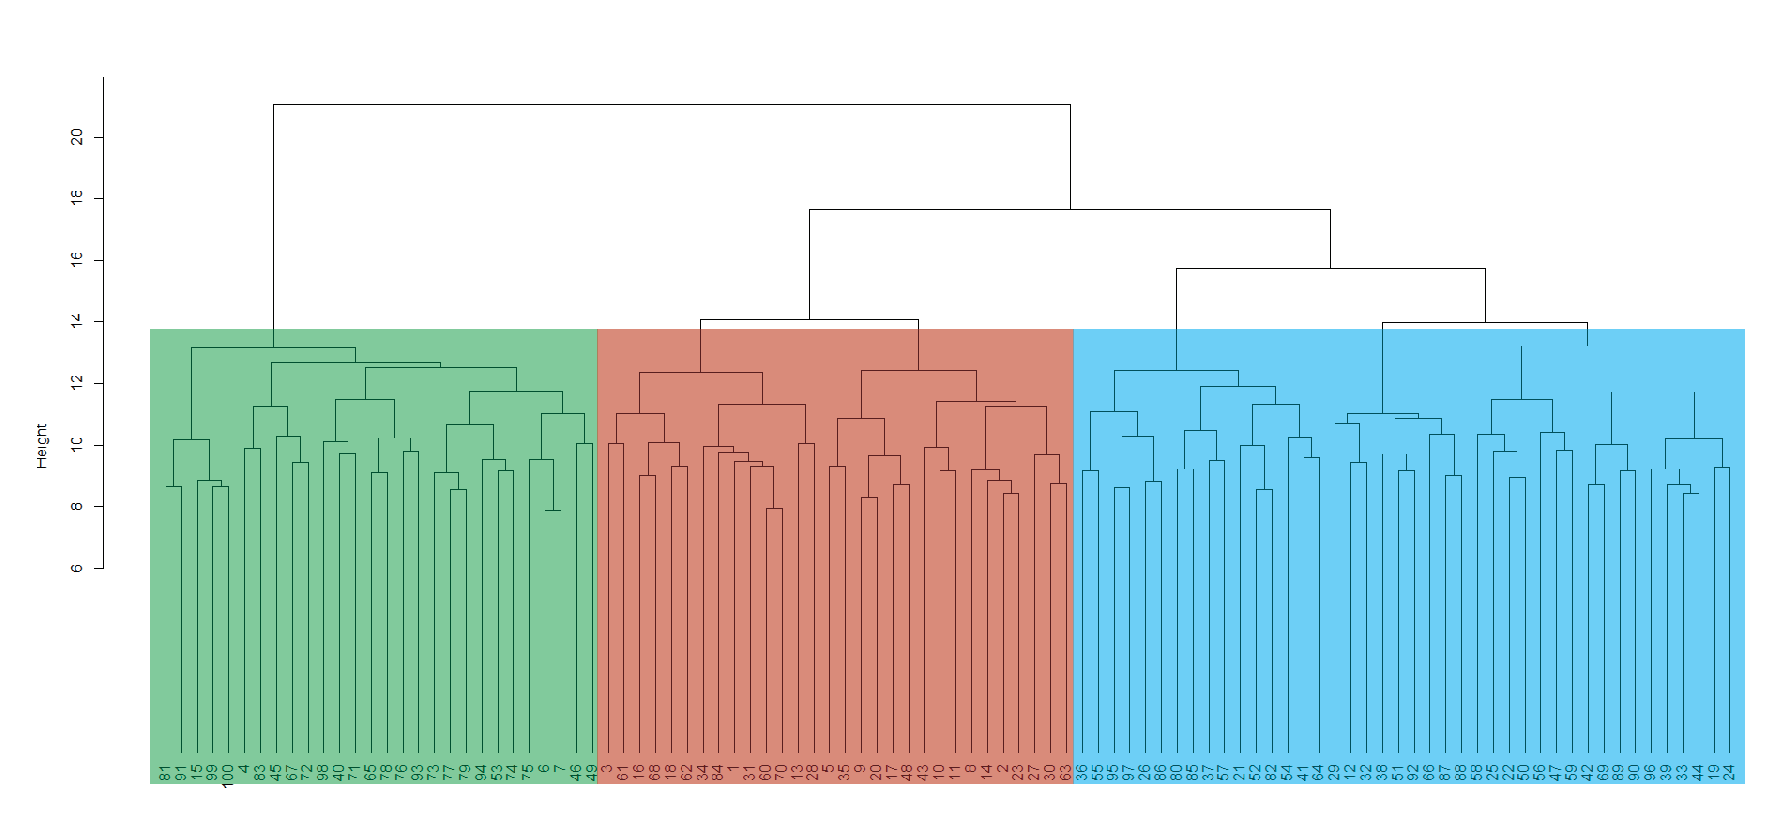
\includegraphics[width=5cm]{clusterresults.pdf}
\caption{学生100人分のクラスター分析}\label{学生100人分のクラスター分析}
\end{figure}


\section{考察}
各色ごとの特徴は図1に記載する.図1の中で近しい人達の個人データをまとめ共通事項を抽出した.例えば緑色の75,6,7,46,49の5人は,AO入試で入学した人たちで進級に若干不安な考えを持っている群衆である.このように細かい群衆で見るとどのような考え方や意識の学生なのか理解できる.
\section{結論}
群衆の特徴をまとめることができる分析手法を提案できた.調査報告書の手法との相違点は全ての項目を絡めた点である.全ての項目を絡めたことにより人の習性や行動パターンも明らかにした.

    

\bibliographystyle{junsrt}
\bibliography{biblio}%「biblio.bib」というファイルが必要.
\end{document}
